\documentclass[12pt,letterpaper]{article}

\usepackage{graphicx,color}
\usepackage{natbib}
\usepackage{amsmath,amsfonts,amsthm,amssymb,euscript,mathrsfs,url,bbm}
\usepackage{algorithmic, stmaryrd}
\usepackage[tight]{subfigure}
\usepackage{psfrag}
\usepackage{multirow}
\usepackage{fancyhdr,lastpage}
\usepackage{verbatim}
\usepackage{varwidth}

\newcommand{\vect}[1]{\boldsymbol{#1}}
\newcommand{\matr}[1]{\boldsymbol{#1}}
\DeclareMathOperator*{\argmin}{arg\,min}
\DeclareMathOperator*{\argmax}{arg\,max}
\newcommand*{\vertbar}{\rule[1ex]{0.5pt}{2.5ex}}
\newcommand*{\horzbar}{\rule[.5ex]{2.5ex}{0.5pt}}


% some formatting from http://www.tedpavlic.com/post_homework_tex_example.php:
% In case you need to adjust margins:
\topmargin=-0.45in
\evensidemargin=-0.1in
\oddsidemargin=-0.4in
\textwidth=7.3in
\textheight=9.0in
\headsep=0.25in
\headheight=30pt

% Setup the header and footer
\pagestyle{fancy}
\lhead{CS66: Machine Learning \hfill \hmwkTitle:\ Due April 5, 2019} % TODO change date
\cfoot{}
\rfoot{Page\ \thepage\ of\ \protect\pageref{LastPage}}
\renewcommand\headrulewidth{0.4pt}
\renewcommand\footrulewidth{0.4pt}

\newcommand{\R}{\mathbb{R}}
\newcommand{\Z}{\mathbb{Z}}
\newcommand{\N}{\mathbb{N}}
\newcommand{\Q}{\mathbb{Q}}

\newcommand{\var}{\mathop{\mbox{Var}}}
\newcommand{\cov}{\mathop{\mbox{Cov}}}
\newcommand{\grad}{\nabla}

\newcommand{\sCol}[1]{\mathscr{#1}}
\newcommand{\sCmp}[1]{#1^{\text{c}}}
\newcommand{\sigF}{\sigma\text{-field}}

\newcommand{\iidsim}{\stackrel{\mathrm{iid}}{\sim}}

\newenvironment{centerverbatim}{%
  \par
  \centering
  \varwidth{\linewidth}%
  \verbatim
}{%
  \endverbatim
  \endvarwidth
  \par
}

\DeclareMathOperator{\leb}{Leb}
\DeclareMathOperator{\cl}{cl}
\DeclareMathOperator{\Ber}{Ber}
\DeclareMathOperator{\Poi}{Poi}
\DeclareMathOperator{\Gam}{Gam}
\DeclareMathOperator{\Bin}{Bin}
\DeclareMathOperator{\IG}{IG}
\DeclareMathOperator{\Max}{Max}
\DeclareMathOperator{\Exp}{Exp}
\DeclareMathOperator{\Nor}{Normal}
\DeclareMathOperator{\Uni}{Unif}
\DeclareMathOperator{\Par}{Pareto}
\DeclareMathOperator{\Dir}{Dir}
\DeclareMathOperator{\Bet}{Beta}
\DeclareMathOperator{\Cau}{Cau}
\DeclareMathOperator{\TN}{TN}
\DeclareMathOperator{\Null}{Null}

\DeclareMathOperator{\E}{E}

\newcommand{\probnumber}[1]{\noindent\textbf{(#1)}}

\newcommand{\hmwkTitle}{Lab 6}
\begin{document}
% TODO: begin here

\section*{SVM Problem Set}
\noindent {\em Names:}

\begin{enumerate}

% QUESTION 1
\item Prove that the {\em geometric margin} (physical distance between the point and the hyperplane) for a given example $(\vec{x}_i, y_i)$ and a given hyperplane ($\vec{w} \cdot \vec{x} + b = 0$) is
\[ \gamma_i = y_i \left(\frac{\vec{w}}{\|\vec{w}\|} \cdot \vec{x}_i + \frac{b}{\|\vec{w}\|}\right) \]
We did a few of the steps in class -- your task here is to explain those steps in your own words (a picture would be very helpful) and fill in the missing steps. 

% TODO uncomment below to put your solution in blue
%{\color{blue}{Solution:}}
\vspace{3mm}


% QUESTION 2
\item The Lagrangian for our SVM problem is
\[ \mathcal{L}(\vec{w}, b, \vec{\alpha}) = \frac{1}{2} \| \vec{w} \|^2 - \sum_{i=1}^n \alpha_i \big[y_i (\vec{w}\cdot \vec{x}_i + b) - 1\big] \]
After we take the gradient with respect $\vec{w}$ and the derivative with respect to $b$, we end up with these two equations
\[ \vec{w} = \sum_{i=1}^n \alpha_i y_i \vec{x}_i \quad , \quad \sum_{i=1}^n \alpha_i y_i = 0 \]

Use these equations to demonstrate that
\[ \mathcal{L}(\vec{w}, b, \vec{\alpha}) = \sum_{i=1}^n \alpha_i - \frac{1}{2} \sum_{i=1}^n \sum_{j=1}^n y_i y_j \alpha_i \alpha_j \vec{x}_i \cdot \vec{x}_j  \]

(The RHS is what we redefine as $W(\vec{\alpha})$, since it no longer depends on $\vec{w}$ and $b$.)

\vspace{3mm}

% QUESTION 3
\item Why is the ``max of the mins'' always less than or equal to the ``min of the maxs''?  In other words, let $f(x,y)$ be a function of two variables -- why is
\[ \max_x \ \min_y f(x,y) \leq \min_y \ \max_x f(x,y) \ ?\]
Hint: imagine a matrix of $f(x,y)$ values, with $x$ denoting the row and $y$ denoting the column.  Think about first fixing the row and finding the min over all $y$ values in that row.  Then do that for each row and take the max.  Then reverse the steps.

\vspace{3mm}

% QUESTION 4
\item {\em Challenge} (not optional but worth few points): After finding the optimal alpha values $\alpha_i^*$ (for $i=1,\cdots,n$), we can find the optimal weight vector $\vec{w}^*$.
%\[ \vec{w}^* =  \sum_{i=1}^n \alpha_i^* y_i \vec{x}_i \]
Demonstrate that the optimal bias is
\[ b^* = -\frac{1}{2} \left( \max_{i:y_i = -1} \vec{w}^* \cdot \vec{x}_i  + \min_{i:y_i = 1} \vec{w}^* \cdot \vec{x}_i \right) \]
Hint: think about the constraints in our optimization problem after we forced $\hat{\gamma} = 1$. The bias only shifts our hyperplane up and down (doesn't change its direction), so we want to move it to the ``middle'' of the support vectors from each class.

\newpage

% QUESTION 4
\item The goal of this question is to gain some intuition about SVMs through a concrete example.  Consider the 6 examples shown below from two classes (+1, $-$1). 
\begin{figure}[h!]
\center
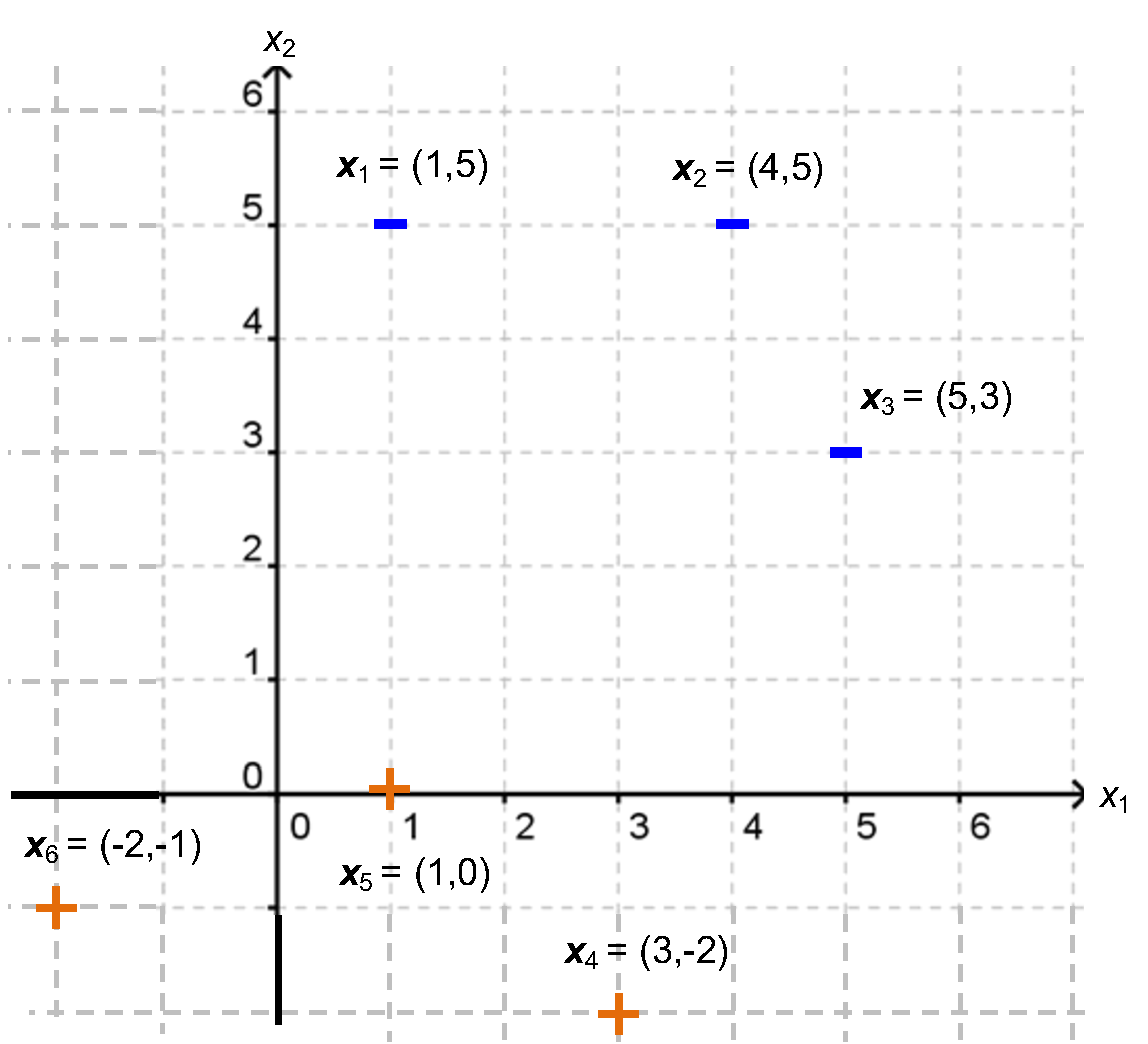
\includegraphics[width=100mm]{svm_ex.pdf}
\end{figure}

\begin{enumerate}
\item Using your knowledge of what the maximum margin hyperplane means, draw the ``best'' hyperplane on the figure above.
\vspace{3mm}

\item What is an {\em equation} (in terms of the axes $x_1$ and $x_2$) that describes this optimal hyperplane?
\vspace{3mm}

\item Which of the $\vec{x}_i$'s are support vectors?
\vspace{3mm}

\item Given that the weight vector is orthogonal to the hyperplane, write $\vec{w}$ as
\[ \vec{w} = a \left[\begin{array}{c}w_1 \\ w_2 \end{array}\right] \]
for some concrete $w_1$ and $w_2$ and some unknown constant $a$. In other words, find the direction of the weight vector.
\vspace{3mm}

\item Using the fact that the functional margin $\hat{\gamma} = 1$ (i.e. $\hat{\gamma}_i = 1$ for support vectors), solve for this constant $a$ and the bias $b$. At this end of this part you should have numerical values for the optimal weight vector $\vec{w}^*$ and the optimal bias $b^*$. 
\vspace{3mm}

\item Finally, using the fact that $\vec{w} = \sum_{i=1}^n \alpha_i y_i \vec{x}_i$ and $\sum_{i=1}^n \alpha_i y_i = 0$, find the optimal $\alpha_i^*$ for $i=1, \cdots, 6$.

\end{enumerate}

\end{enumerate}

\end{document}
